\chapter{Café and Special Diet}
\section{Team Structure}
Ahead of camp, the Café and Special Diets team was composed of Joe Bowler and Chris Bowler. They had originally planned to be an offshoot of the food team - working towards the common goal of feeding people, however due to the elevated support needs of the Food Team, they were unable to solely exist out of the café. This led to the Special Diets division operating from the Main Food Distribution Marquee. \\

On camp, Joe took a lead on the café, while Chris focused on the Special Diets. They had support from Caitlyn McArthur, who volunteered initially as part of the Special Diets team and ended up working more in the Café.\\

Within the Café, Beth was the fantastic Maître D, Alex and Ash were amazing chefs de partie, Caitlyn did a wonderful job as Front of House, and Laurence was the perfect Venturer guinea pig / mascot!\\

Several people dropped out in the lead up to camp and unfortunately none of the remaining onsite volunteers had capacity to do any pre-event organising. This put a lot of pressure on Joe and some areas suffered, including ordering food before camp and organising the café takeovers.\\

A big contributing factor to short staffing was the lack of 16-17 yr old volunteers, without them we needed the whole core café team to open up the café. This drastically reduced the amount of time we could be open and ment that volunteers did not get time off. \\

The team worked amazingly well and we had such a good time working together in the kitchen. Joe noted ``I'm really proud of everyone who worked in the café and space we created!''
\subsection{Evaluation of Team Structure}
Joe and Chris took on too much and were definitely overworked, it's only through the support of their friends and volunteers that they made it look good. 
The café had reduced opening times and menu choices because of the volunteer issues. However the café was very busy from the Monday onwards all the way through.\\

The special diets team was structured poorly. It's a work in progress concept and we're certainly discovering what not to do and slowly discovering what to do.
Village KPs are much more likely to accept the support in the form of ingredients and recipes. They do not want someone else cooking the food outside the village. 
People with special diets are not keen for food to be prepared without seeing it be cooked and see the packaging. People are very much on edge about allergies and the consequences of messing up. Chris only cooked 2 meals outside the KPs doing it themselves (1 meal each for 2 people). \\

Special Diets structure needs to  involve the village KPs at a much earlier stage. Chris spoke to the leaders more than the young people that needed help (leaders of these young people were often on the village KP team) and ordered food to supplement for special diet needs. 

\subsection{Support Ahead of Camp}
The team did not feel well-supported in the lead-up to camp. They should have reached out to coordination / volunteer support to help the KPs, as they could not do their job without the KPs sorting some things first (the menu, for example). But it didn't feel there was capacity in the wider team to help with either this or special diets. A longer lead-in to the event would definitely have helped here as it would have allowed for certain things to be set far out in advance, thus enabling subsequent activities to be less time-compressed.

\subsection{Team Redesign}
For the Café team, a massive difference would be made from the number of people in the team increasing. Not only would this reduce the burden on individuals during the camp, it would also enable more people to be involved in the picking of the merchandise - thus allowing a richer variety of food and drinks, which people are more likely to want. As it stood, the menu was often decided while looking at stock in Bookers Wholesale. The Café team would also have benefited from using the bakers (which the food team were using for desserts) for baked supplies.\\

For the Special Diets team, a dedicated person is needed who can go around the site and talk to different people, talking them through the menu (this person needs to have an intimate knowledge of the menu). This would be supported by an individual / team who can cook as and when needed. At a Venturer Camp sized event - it would work to do this with two people, as their only role on Camp; obviously this figure would need to be scaled up as the camp grows. Part of the core role of a future Special Diets team would be to educate Village KPs on how to handle allergies before camp. It would also be nice for the Special Diets team to facilitate a caucus between Village KPs and Parents of Allergy Kids. 

\section{Supporting Events}
\subsection{Pre-Camp}
The Café \& Special Diets Online Pre-Camp event had very low attendance, with the only person turning up not knowing about allergies. Joe and Chris enjoyed the session as it gave them a good chance to get their words in order about allergies and catering for them.\\

Joe and Chris both attended the On-Site Pre-Camp weekend which they found useful. They enjoyed seeing the spaces physically and being able to visualise the Café space! It did highlight things which hadn't yet been considered - however this was useful. The most useless part of the weekend for them was going on the Car Park walk. 

\subsection{Working Week}
Joe and Chris both came to Working Week, where for a good proportion of the time they helped with the manual labour, such as putting tents up. They also used the time to set up their spaces, including moving an oven, clearing out the Café and furnishing it as they wished. There was also some time spent travelling to the local pub to use their internet to do Special Diets Internet Activities, however this could have been done in advance if there was capacity to do so. 
\subsection{Takedown}
Joe and Chris both came to some of Takedown. They helped to clear down their spaces, which due to understaffing was ``a complete mess''. This is something which should be managed better on camps, or even as part of the last day.  Everyone was exhausted, suggested to recruit people for takedown only.

\section{On-Camp Operations}
\subsection{Daily Structure}
The Café \& Special Diets Team was one of the, if not the, most overworked teams on site. To quote their evaluation interview, their days consisted of ``get up, work, work, work, work, work, sleep''.\\

Joe spent all of his time either in the Café, or when it wasn't open - offsite buying for the café or making food for the café.\\

Chris would wake up early to meet the bakers, then run the KP meeting (something which he stood in for due being the best personality to run them, in the future if there's not someone in the KP team who feels confident enough to run a whole group meeting - run them as a series of 1:1s). He would spend the rest of his day dashing around site dealing with Special Diet meals, working in the café and delivering food to different bits of the site by bike.
\subsection{Time Off}
Both Joe and Chris were able to get some time off in the evenings. Joe didn't get a complete day off, however had an afternoon off and Chris managed an entire day off. 
\subsection{Support}
Support from the coordinator and cabin team was good, but Volunteer Support engagement was limited. They should have visited teams to check in rather than expecting teams to go to them. PEB was deemed not accessible, too big so not cosy, and should have had light evening programme for chilling after a long day.

\section{Café \& Special Diets Team Specific Insights}
\begin{figure}[h]
    \centering
    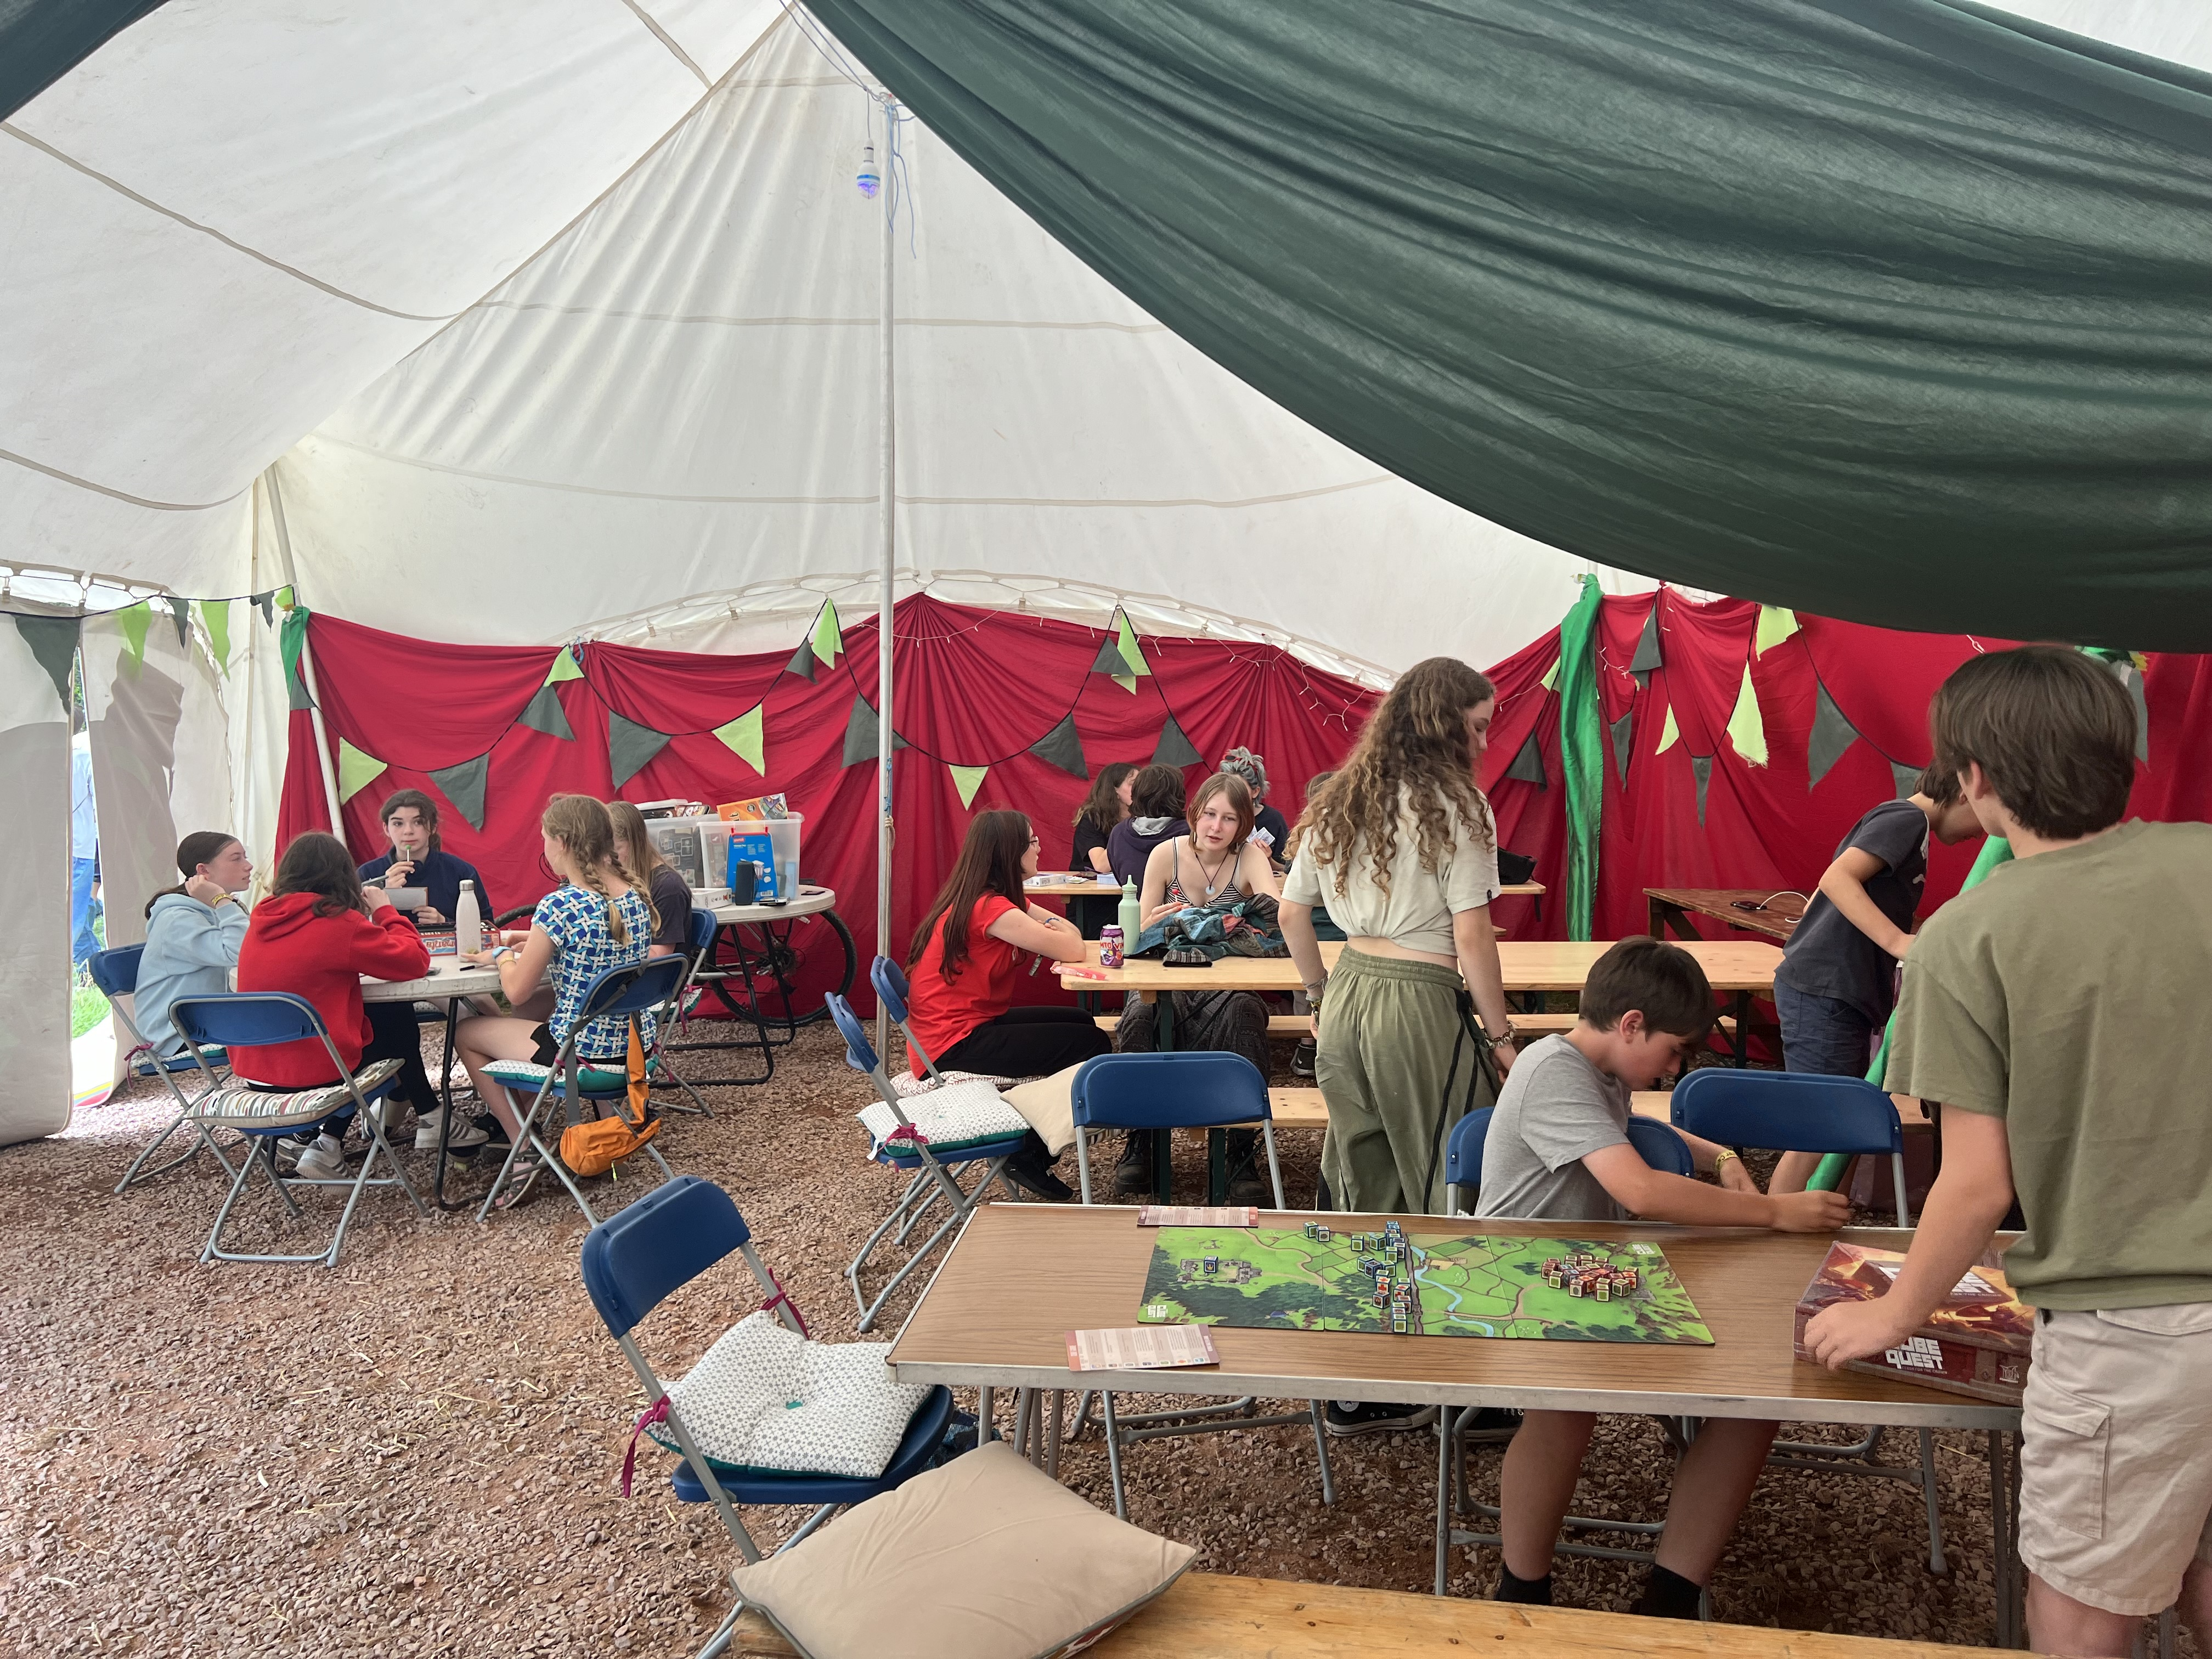
\includegraphics[width=0.8\textwidth]{assets/cafe-full-swing-ab.jpeg}
    \caption{Café in full swing (\textit{AB})}
\end{figure}
\subsection{Challenges Experienced}
Due to limited time for pre-event organising, plans which had been laid for running café takeovers and ordering food, were unable to happen. The café takeovers were unable to happen properly due to not having enough time to plan them.\\

The lack of 16 \& 17 year old volunteers, due to the expanded age ranges of the camp, impacted the core team's ability to open the café. This reduced opening hours and therefore reduced income from the café.
\subsection{Improvements for Next Time}
With a longer lead time for the next camp, the menu and ingredients will be finalised earlier. This will then enable the Special Diets team to begin planning with Village KPs around what meals they will need support with.\\

The Café needs more volunteers to enable it to open for longer hours. As well as the team needing support with sorting things that aren't specifically Café or Special Diets, however directly impact their operations. This includes things such as sourcing an oven, dealing with the gas, and sorting food refrigeration.
\subsection{Miscellaneous Insights}
Joe and Chris brought their own bikes to the event. This enabled them to travel around the site quicker. This is something which all core team should be encouraged to do, if possible. It was especially useful for the Café team where they were cooking in the Koodoo kitchen, near pitch 1, and serving from the Café on Pitch 5. \\

Lots of ideas have been thought about for the next incarnation of the Allergy Kitchen. These mostly include resources such as: special diets cookbooks and blank templates for meals. This would make the Special Diets Kitchen more efficient. \\

The Café team struggled with the use of VCoin. They have suggested not to repeat it in the future. VCoin is explored in greater detail elsewhere in this report.
\subsection{Future Focus}
Future events should come with an emphasis on upskilling village KPs, this will enable them to require less hand holding around a centrally devised menu as well as building the next generation of Central KPs. Working with suppliers to develop relationships with them should be a top priority, as well as working with the central Woodcraft Folk staff team to support this. The team commented that working with the Head of Resources was extremely helpful, and having this support sooner would have been helpful. It's also important to engage the Wider Team in the planning process, not just in the last few weeks.\\

It is also important to focus on creating comfortable workspaces, as well as comfortable spaces on camp. This was a particular challenge at Biblins where many of the semi-permanent marquees, including the Café Marquee, are site on a gravel hard standing.

\subsection{Popular Café Items}
The café didn't record sales. Generally speaking: cans of drinks, biscuits and cheese toasties were popular. These were all served in a way such that they could be taken out of the café, to other parts of the central area - perhaps contributing to their popularity. The Café team believes that if they had disposable cups, people would have bought drinks from the big bottles, at a lower cost to us therefore lower price to them, as they liked being able to take drinks away.\\

The café aimed to sell products which weren't available in Villages for snacks or as part of the main menu - this works well as people are enticed to the café to find treats. 
\subsection{How Special Diets Worked}
Using the booking data we designated attendees into categories of how much support they might need with diets on a 1-4 system.
\begin{enumerate}
    \item People with needs that are easy to cater to, e.g. don't like mushrooms, melon allergy, not too spicy. These people will just have a note sent to the village KP so they are aware. These people shouldn't need any outside of village intervention
    \item People with diets that will require alternative ingredients, e.g Milk intolerance. These people will have alternatives such as plant milks and vegan cheeses provided by the central KP team
    \item People who have special needs or combination allergies, e.g Diabetic, celiac, vegan+quorn allergy. These people need their own action plans like separate storage and food prep tables or may need some special alternative foods bought by the SDT. We're aiming for all this food to be prepared in the village. 
    \item People with severe allergies, multiple combination allergies, or a special diet. They may require multiple meals to be altered or an entirely different diet planned for them on camp. There were 10 people in this category. substitutions to the core menu, custom meal plans, or pre-packaged meals
\end{enumerate}
\subsection{Specific Diets We Worked With}
\subsubsection{Combination Allergies}
Combination allergies are a major challenge for finding substitution ingredients. For example, A vegan with a soya allergy cannot eat meat free sausages and yet the alternative cannot be eaten by the vegan with a pulses allergy. 
\subsubsection{Elimination Diets}
An elimination diet is a dietary approach that involves temporarily removing certain foods or food groups from your eating routine to identify potential food intolerances or sensitivities. It is often used as a diagnostic tool to determine which specific foods may be causing adverse reactions or symptoms in an individual. 
\subsubsection{Diabetic Diets}
Diabetic support is something that we've just started looking into. We can provide glucose boosting snacks and drinks, and make nutrition information available for insulin calculations.
\subsubsection{Gastro Health Conditions}
Gastrointestinal (GI) health conditions encompass a wide range of disorders that affect the digestive system, including the oesophagus, stomach, intestines, liver, gallbladder, and pancreas. These conditions can have varying impacts on diet and nutritional needs. These can include GERD, IBD, IBS, Celiac Disease, and Liver Disease 
\subsubsection{ARFID and Autism}
Avoidant/Restrictive Food Intake Disorder can be described as a clinically significant form of "fussy eating" or selective eating. While many young people and adults may display some level of picky eating behaviour, ARFID goes beyond typical picky eating and involves severe and persistent limitations in food intake that significantly impact a person's physical health and daily functioning. Many campers with ASD have eating difficulties that can manifest as selective eating or ARFID-like behaviours. 
